\chapter{Примеры задач}
\selectlanguage{russian}
\taskinit

В данном разделе приведены примеры задач, которые использовались на контрольных работах в МФТИ по курсу <<Защита информации>> в 2011--2015 годах.

\section{Математические основы}
\tasksection

\tasknumber Найдите общее количество и перечислите генераторы аддитивной циклической группы $\mathbb{Z}_{33}$ с операцией в виде сложения чисел по модулю 33.
\medbreak
\textbf{Ответ:} 20: [1, 2, 4, 5, 7, 8, 10, 13, 14, 16, 17, 19, 20, 23, 25, 26, 28, 29, 31, 32].
\bigbreak

\tasknumber Вычислить в поле Галуа $GF\left( {2^{5} } \right)$, $m\left( x \right) = x^{5} + x^{3} + x^{2} + x + 1$, следующее значение: $28 \times 29 + 23^2$. Многочлены заданы как десятичное представление двоичных коэффициентов, свободный член многочлена соответствует младшему биту двоичного представления. В ответе привести в десятичном представлении результаты умножения, возведения в степень и сложения.
\medbreak
\textbf{Решение:}
\begin{itemize}\itemsep1pt \parskip0pt \parsep0pt
	\item $a = "28" \Rightarrow a\left( x \right) = x^{4} + x^{3} + x^{2}$;
	\item $b = "29" \Rightarrow b\left( x \right) = x^{4} + x^{3} + x^{2} + 1$;
	\item $c = "23" \Rightarrow c\left( x \right) = x^{4} + x^{2} + x + 1$;
	\item $a \left( x \right) \times b \left( x \right) = x^{4} + x^{3} + x + 1 \Rightarrow a \times b = "27"$;
	\item $c \left( x \right)^2 = x^{4} + x^{3} + x^{2} \Rightarrow c^2 = "28"$;
	\item $result\left( x \right) = x^{2} + x + 1 \Rightarrow result = "7"$.
\end{itemize}
\medbreak
\textbf{Ответ:} <<27>>; <<28>>; <<7>>.
\bigbreak

\tasknumber Вычислить в поле Галуа $GF\left( 27 \right)$, $m\left( x \right) = x^{3} + x^{2} + x + 2$, следующее значение: $26 \times 11 + 25^2$. Многочлены заданы как десятичное представление троичных коэффициентов, свободный член многочлена соответствует младшему биту троичного представления. В ответе привести в десятичном представлении результаты умножения, возведения в степень и сложения.
\medbreak
\textbf{Решение:}
\begin{itemize}\itemsep1pt \parskip0pt \parsep0pt
	\item $a = "26" \Rightarrow a\left( x \right) = 2 x^{2} + 2 x + 2$;
	\item $b = "11" \Rightarrow b\left( x \right) = x^{2} + 2$;
	\item $c = "25" \Rightarrow c\left( x \right) = 2 x^{2} + 2 x + 1$;
	\item $a \left( x \right) \times b \left( x \right) = x^{2} + 1 \Rightarrow a \times b = "10"$;
	\item $c ^2\left( x \right) = x + 2 \Rightarrow c^2 = "5"$;
	\item $result\left( x \right) = x^{2} + x \Rightarrow result = "12"$.
\end{itemize}
\medbreak
\textbf{Ответ:} <<10>>; <<5>>; <<12>>.
\bigbreak

\tasknumber Используя алгоритм быстрого возведения в степень (с помощью разложения показателя степени по степеням двойки по схеме <<слева направо>>), вычислить ${175}^{235} \mod {257}$.
\medbreak
\textbf{Решение:}
\begin{itemize}\itemsep1pt \parskip0pt \parsep0pt
	\item двоичная форма записи степени: $235_{10} = 11101011_{2}$;
	\item полное выражение для вычисления: $(((((((1 \times {175}^1)^2 \times {175}^1)^2 \times {175}^1)^2 \times {175}^0)^2 \times {175}^1)^2 \times {175}^0)^2 \times {175}^1)^2 \times {175}^1\mod 257$;
	\item шаг \No1: $1^2 \times 175 \mod 257  = 175$;
	\item шаг \No2: $175^2 \times 175 \mod 257 = 154$;
	\item шаг \No3: $154^2 \times 175 \mod 257 = 7$;
	\item шаг \No4: $7^2 \mod 257 = 49 \mod 257 = 49$;
	\item шаг \No5: $49^2 \times 175 \mod 257 = 237$;
	\item шаг \No6: $237^2 \mod 257 = 143$;
	\item шаг \No7: $143^2 \times 175 \mod 257 = 107$;
	\item шаг \No8: $107^2 \times 175 \mod 257 = 3$.
\end{itemize}
\medbreak
\textbf{Ответ:} 3.
\bigbreak

\section{Общие определения и теория}
\tasksection

\tasknumber Рассмотрим множество паролей, состоящих из 12 строчных и заглавных латинских букв, а также цифр.
\begin{itemize}\itemsep1pt \parskip0pt \parsep0pt
\item Каков размер этого множества?
\item Сколько времени потребуется на взлом шифротекста, зашифрованного данным паролем, если предположить, что во взломе участвуют все компьютеры мира (7~млрд.), а средний компьютер перебирает 300~000 паролей в секунду?\footnote{См. скорости перебора MD5-хэшей\index{хэш-функция!MD5} на странице \texttt{http://openwall.info\hspace{0pt}/wiki\hspace{0pt}/john\hspace{0pt}/benchmarks}}
\item Каковы затраты электроэнергии в денежном эквиваленте, если средний компьютер потребляет мощность 400~Вт, а стоимость 1~кВт$\times$час составляет 4,68~рубля?
\end{itemize}
\medbreak
\textbf{Решение:}
\begin{itemize}\itemsep1pt \parskip0pt \parsep0pt
	\item общее количество символов: $26 + 26 + 10 = 62$;
	\item общее количество паролей: $62^{12} \approx 3{,}226\times 10^{21}$;
	\item время на перебор: $62^{12} / (3 \times 10^5) / (7 \times 10^9 ) \approx 1{,}54 \times 10^{6}$ сек.;
	\begin{itemize}\itemsep1pt \parskip0pt \parsep0pt
		\item в минутах: $\approx 25605$;
		\item в часах: $\approx 427$;
		\item в днях: $\approx 18$;
	\end{itemize}
	\item стоимость: $427 \times (7 \times 10^9 ) \times 0{,}4 \times 4{,}68 \approx 5{,}59 \times 10^{12}$ руб.
\end{itemize}
\medbreak
\textbf{Ответ:} паролей $3{,}226 \times 10^{21}$; на перебор нужно $1{,}54 \times 10^6$ секунд ($\approx 18$ дней); затраты -- 5,6 триллиона рублей.
\bigbreak

\tasknumber Источник открытого текста характеризуется случайной величиной $X$, принимающей два значения $x_1$ и $x_2$ с вероятностями $p \left( x = x_1 \right) = 1/5$ и $p \left( x = x_2 \right) = 4/5$ соответственно. Источник ключей характеризуется случайной величиной $Z$, независимой от величины $X$, принимающей два значения $z_1$ и $z_2$ с вероятностями $p \left( z = z_1 \right) = 1/6$ и $p \left( z = z_2 \right) = 5/6$ соответственно. Функция шифрования $E_{z} \left( x \right)$ задаётся следующими правилами: $\left( x_1, z_1 \right) \to y_1$, $\left( x_1, z_2 \right) \to y_2$, $\left( x_2, z_1 \right) \to y_2$, $\left( x_2, z_2 \right) \to y_1$.
\begin{enumerate}\itemsep1pt \parskip0pt \parsep0pt
	\item Найдите собственную информацию каждого из сообщений открытого текста в битах.
	\item Найдите энтропию источника сообщений, источника ключей и шифротекста в битах.
	\item Найдите взаимную информацию открытого текста и ключа в битах.
	\item Найдите взаимную информацию открытого текста и шифротекста в битах.
	\item Найдите взаимную информацию ключа и шифротекста в битах.
	\item Найдите апостериорное распределение вероятностей открытого текста для обоих вариантов перехваченных злоумышленником шифротекстов $y_1$ и $y_2$. Используя вычисленные значения, определите, является ли данная шифросистема абсолютно надёжной. Если нет, то что в данной криптосистеме необходимо поменять? Покажите, что апостериорные вероятности после доработки будут удовлетворять необходимым требованиям абсолютно надёжной криптосистемы.
\end{enumerate}
\medbreak
\textbf{Ответ:}
\begin{itemize}\itemsep1pt \parskip0pt \parsep0pt
	\item $I \left( x_1 \right) = \log_2 5 = 2{,}322$ бит; $I \left( x_2 \right) = \log_2 5/4 = 0{,}322$ бит;
	\item $H \left( X \right) = 0{,}722$ бит; $H \left( Z \right) = 0{,}650$ бит; $H \left( Y \right) = 0{,}881$ бит;
	\item $I \left( X ; Z \right) = 0$ бит; $I \left( X; Y \right) = 0{,}231$ бит; $I \left( Y; Z \right) = 0{,}159$ бит;
	\item $p \left( x_1 | y_1 \right) = 1/21$; $p \left( x_2 | y_1 \right) = 20/21$; $p \left( x_1 | y_2 \right) = 5/9$; $p \left( x_2 | y_2 \right) = 4/9$; не является.
\end{itemize}

\section{КСГПСЧ и потоковые шифры}
\tasksection

\tasknumber Привести следующие два элемента последовательности, сформированной линейным конгруэнтным методом, если предыдущие 3 элемента последовательности такие: 348, 65, 139, а все вычисления выполняются в поле $\mathbb{F}_{499}$.
\medbreak
\textbf{Решение:}
\begin{itemize}\itemsep1pt \parskip0pt \parsep0pt
	\item используя предыдущие значения выхода генератора, строим систему уравнений:
		\[\left\{ {\begin{array}{*{20}c}
		348 \cdot a + c = 65 \mod 499 \\
		65 \cdot a + c = 139 \mod 499 \\
		\end{array} } \right. ;\]
	\item из системы уравнений находим $a = 467$ и $c = 223$;
	\item используя найденные значения, находим следующие элементы последовательности;
	\begin{itemize}\itemsep1pt \parskip0pt \parsep0pt
		\item $x_{3} = a x_{2} + c \mod m = 467 \cdot 139 + 223 \mod 499 = 266$;
		\item $x_{4} = a x_{3} + c \mod m = 467 \cdot 266 + 223 \mod 499 = 194$.
	\end{itemize}
\end{itemize}
\medbreak
\textbf{Ответ:} 266, 194.
\bigbreak

\tasknumber Приведите \emph{предыдущие} 5 бит выхода генератора псевдослучайной последовательности, основанного на регистре сдвига с линейной обратной связью, если известно, что характеристический полином регистра — $m\left(x\right)=x^{5} + x^{3} + 1$ (см. рис.), а дальнейшая последовательность такова: $1, 1, 0, 1, 0, 1$.
\begin{center}
	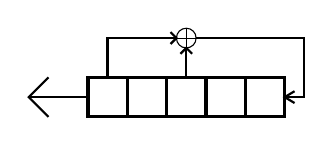
\begin{tikzpicture}[scale=0.05]
		\draw[black,very thick] (30,30) -- (30,40) -- (40,40) -- (40,30) -- (30,30) -- (30,40);
		\draw[black,thick] (35,40) -- (35,50) -- (35,50) -- (37.5,50);
		\draw[black,very thick] (40,30) -- (40,40) -- (50,40) -- (50,30) -- (40,30) -- (40,40);
		\draw[black,very thick] (50,30) -- (50,40) -- (60,40) -- (60,30) -- (50,30) -- (50,40);
		\draw[black,thick] (55,40) -- (55,47.5);
		\draw[black,thick] (53.5,46) -- (55,47.5) -- (56.5,46);
		\draw[black,thick] (37.5,50) -- (52.5,50);
		\draw[black,thick] (51,51.5) -- (52.5,50) -- (51,48.5);
		\draw (55,50) circle [radius=2.5];
		\draw[black] (52.5,50) -- (57.5,50);
		\draw[black] (55,47.5) -- (55,52.5);
		\draw[black,very thick] (60,30) -- (60,40) -- (70,40) -- (70,30) -- (60,30) -- (60,40);
		\draw[black,very thick] (70,30) -- (70,40) -- (80,40) -- (80,30) -- (70,30) -- (70,40);
		\draw[black,thick] (57.5,50) -- (85,50) -- (85,35) -- (80,35);
		\draw[black,thick] (82.5,36.5) -- (80,35) -- (82.5,33.5);
		\draw[black,thick] (30,35) -- (15,35);
		\draw[black,thick] (20,30) -- (15,35) -- (20,40);
	\end{tikzpicture}
\end{center}
\medbreak
\textbf{Решение.}
\begin{itemize}\itemsep1pt \parskip0pt \parsep0pt
	\item Из коэффициентов многочлена $m\left(x\right)$ получаем формулу предыдущего элемента:
		\[ m\left(x\right) = \sum\limits_{i = 5 \dots 1} {a_i x^i } + 1 = x^{5} + x^{3} + 1; \]
		\[ b_0 = a_5 b_5 \oplus \dots \oplus a_1 b_1 = b_{5} \oplus b_{3}.\]
		Это формула бита, который на следующей итерации станет битом $b_1$, то есть значение функции обратной связи регистра;
	\item $b_5 = b_0\oplus b_{3}$ -- формула выходного бита, если известны остальные биты и значение функции обратной связи;
	\item За счёт последних 5 бит выхода восстанавливаем состояние регистра $\overrightarrow{s_{1}}=\left(b_{1}, b_{2}, b_{3}, b_{4}, b_{5}\right) = \left(1, 0, 1, 0, 1\right)$. Далее начинаем отматывать время назад.
	\item $\overrightarrow{s_{1}}=\left(1, 0, 1, 0, 1\right)$. $\overrightarrow {s_{0}} = \left(0, 1, 0, 1, ? \right)$ и $b_0 = 1$. \\
		$b_5 = b_0\oplus b_{3}=1 \oplus 0=1$. $\overrightarrow{s_{0}}=\left(0, 1, 0, 1, 1\right)$. \\
		Выход — 1;
	\item $\overrightarrow{s_{0}}=\left(0, 1, 0, 1, 1\right)$. $\overrightarrow {s_{-1}} = \left(1, 0, 1, 1, ? \right)$ и $b_0 = 0$. \\
		$b_5 = b_0\oplus b_{3}=0 \oplus 1=1$. $\overrightarrow{s_{-1}}=\left(1, 0, 1, 1, 1\right)$. \\
		Выход — 1;
	\item $\overrightarrow{s_{-1}}=\left(1, 0, 1, 1, 1\right)$. $\overrightarrow {s_{-2}} = \left(0, 1, 1, 1, ? \right)$ и $b_0 = 1$. \\
		$b_5 = b_0\oplus b_{3}=1 \oplus 1=0$. $\overrightarrow{s_{-2}}=\left(0, 1, 1, 1, 0\right)$. \\
		Выход — 0;
	\item $\overrightarrow{s_{-2}}=\left(0, 1, 1, 1, 0\right)$. $\overrightarrow {s_{-3}} = \left(0, 0, 1, 1, ? \right)$ и $b_0 = 0$. \\
		$b_5 = b_0\oplus b_{3}=0 \oplus 1=1$. $\overrightarrow{s_{-3}}=\left(1, 1, 1, 0, 1\right)$. \\
		Выход — 1;
	\item $\overrightarrow{s_{-3}}=\left(1, 1, 1, 0, 1\right)$. $\overrightarrow {s_{-4}} = \left(0, 1, 0, 1, ? \right)$ и $b_0 = 1$. \\
		$b_5 = b_0\oplus b_{3}=1 \oplus 0=1$. $\overrightarrow{s_{-4}}=\left(1, 1, 0, 1, 1\right)$. \\
		Выход — 1;
	\item $\overrightarrow{s_{-4}}=\left(1, 1, 0, 1, 1\right)$. $\overrightarrow {s_{-5}} = \left(0, 1, 1, 0, ? \right)$ и $b_0 = 1$. \\
		$b_5 = b_0\oplus b_{3}=1 \oplus 1=0$. $\overrightarrow{s_{-5}}=\left(1, 0, 1, 1, 0\right)$. \\
		Выход — 0;
	\item Ответ (в порядке выдачи бит генератором): $0, 1, 1, 0, 1$.
	\item Краткое оформление второй части задачи можно увидеть в таблице~\ref{table:task-lfsr-1-short-solution}. Таблица заполняется снизу вверх (так как нам нужны предыдущие биты, а не следующие). Самая последняя строка таблицы соответствует последнему известному состоянию регистра -- последним 5 битам последовательности. Столбцы таблицы связаны формулой $b_{5} \oplus b_{3} = b_0 $. Ответ находится в первых 5 элементах первого столбца. Последние 1 элемента соответствуют вспомогательным битам, данным в решении (первые 1 в последовательности бит из условия).
	\begin{table}[!thb]
		\centering
		\begin{tabular}{ l | c || c c c c c|| c }
		 & & $b_{5}$& $b_{4}$& $b_{3}$& $b_{2}$& $b_{1}$ & $b_0$ \\
		  \hline
		  $\overrightarrow {s_{-5}}$ & 0 & 0 & 1 & 1 & 0 & 1& 1 \\
		  $\overrightarrow {s_{-4}}$ & 1 & 1 & 1 & 0 & 1 & 1& 1 \\
		  $\overrightarrow {s_{-3}}$ & 1 & 1 & 0 & 1 & 1 & 1& 0 \\
		  $\overrightarrow {s_{-2}}$ & 0 & 0 & 1 & 1 & 1 & 0& 1 \\
		  $\overrightarrow {s_{-1}}$ & 1 & 1 & 1 & 1 & 0 & 1& 0 \\
		  $\overrightarrow {s_{0}}$ & 1 & 1 & 1 & 0 & 1 & 0& 1 \\
		  $\overrightarrow {s_{1}}$ & 1 & 1 & 0 & 1 & 0 & 1& $\cdot$ \\
		\hline
		\end{tabular}
		\caption{Краткое оформление решения задачи \No\arabic{task-section}.\arabic{task-number} в виде таблицы}
		\label{table:task-lfsr-1-short-solution}
	\end{table}
\end{itemize}
\medbreak
\textbf{Ответ:} $0, 1, 1, 0, 1$.
\bigbreak

\tasknumber Укажите характеристический полином и приведите следующие 5 бит выхода генератора псевдослучайной последовательности, основанного на регистре сдвига с линейной обратной связью, если известно, что степень характеристического полинома регистра -- $m\left(x\right)$ -- равна 5, а предыдущая последовательность такова: $0, 1, 0, 0, 1, 1, 0, 0, 0, 0, 1$. Порядок бит в последовательности соответствует порядку их генерации РСЛОС.
\medbreak
\textbf{Решение.}
\begin{itemize}\itemsep1pt \parskip0pt \parsep0pt
	\item Каждый бит выходной последовательности есть функция 5 предыдущих выходных бит вида $b_0 = f\left( b_{5} \dots b_1 \right) $. В данных обозначениях $b_{5}$ является наиболее ранним битом, а $b_1$ -- последним, который сгенерировал РСЛОС непосредственно перед генерацией бита $b_0$.  Вид функции задаётся характеристическим многочленом, который и нужно найти.
	\[\begin{array}{l}
		m \left( x \right) = x^{5} +  a_{4} x^{4} + a_{3} x^{3} + a_{2} x^{2} + a_{1} x^{1} +1; \\
		b_{5} \oplus a_{4} b_{4} \oplus a_{3} b_{3} \oplus a_{2} b_{2} \oplus a_{1} b_{1} = b_0. \\
	\end{array}\]
	\[\begin{array}{l}
		f\left(0,1,0,0,1\right) = 1, \\
		f\left(1,0,0,1,1\right) = 0, \\
		f\left(0,0,1,1,0\right) = 0, \\
		f\left(0,1,1,0,0\right) = 0, \\
		f\left(1,1,0,0,0\right) = 0, \\
		f\left(1,0,0,0,0\right) = 1. \\
	\end{array}\]
	\item Это приводит к системе уравнений:
	\[\left\{ {\begin{array}{*{20}c}
		f\left(0,1,0,0,1\right) = 0 \oplus \left( a_{4} \cdot 1\right) \oplus \left( a_{3} \cdot 0\right) \oplus \left( a_{2} \cdot 0\right) \oplus \left( a_{1} \cdot 1\right) = 1 \\
		f\left(1,0,0,1,1\right) = 1 \oplus \left( a_{4} \cdot 0\right) \oplus \left( a_{3} \cdot 0\right) \oplus \left( a_{2} \cdot 1\right) \oplus \left( a_{1} \cdot 1\right) = 0 \\
		f\left(0,0,1,1,0\right) = 0 \oplus \left( a_{4} \cdot 0\right) \oplus \left( a_{3} \cdot 1\right) \oplus \left( a_{2} \cdot 1\right) \oplus \left( a_{1} \cdot 0\right) = 0 \\
		f\left(0,1,1,0,0\right) = 0 \oplus \left( a_{4} \cdot 1\right) \oplus \left( a_{3} \cdot 1\right) \oplus \left( a_{2} \cdot 0\right) \oplus \left( a_{1} \cdot 0\right) = 0 \\
		f\left(1,1,0,0,0\right) = 1 \oplus \left( a_{4} \cdot 1\right) \oplus \left( a_{3} \cdot 0\right) \oplus \left( a_{2} \cdot 0\right) \oplus \left( a_{1} \cdot 0\right) = 0 \\
		f\left(1,0,0,0,0\right) = 1 \oplus \left( a_{4} \cdot 0\right) \oplus \left( a_{3} \cdot 0\right) \oplus \left( a_{2} \cdot 0\right) \oplus \left( a_{1} \cdot 0\right) = 1 \\
	\end{array} } \right.\]
	\[\left\{ {\begin{array}{*{20}l}
		a_{4} \oplus a_{1} = 1 \\
		a_{2} \oplus a_{1} = 1 \\
		a_{3} \oplus a_{2} = 0 \\
		a_{4} \oplus a_{3} = 0 \\
		a_{4} = 1 \\
	\end{array} } \right.\]
	\item Найденные из системы уравнения коэффициенты $\left(a_{4}, a_{3}, a_{2}, a_{1}\right) = \left(1 , 1 , 1 , 0\right)$.
	\item Характеристический полином регистра:
		\[\begin{array}{l}
			m \left( x \right) = x^{5}+ a_{4} x^{4}+ a_{3} x^{3}+ a_{2} x^{2}+ a_{1} x^{1} + 1; \\
			m = x^{5} + x^{4} + x^{3} + x^{2} + 1. \\
		\end{array}\]
	\item Схема РСЛОС приведена на рисунке.
	\begin{center}
		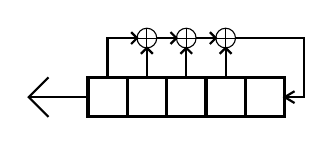
\begin{tikzpicture}[scale=0.05]
			\draw[black,very thick] (30,30) -- (30,40) -- (40,40) -- (40,30) -- (30,30) -- (30,40);
			\draw[black,thick] (35,40) -- (35,50) -- (35,50) -- (37.5,50);
			\draw[black,very thick] (40,30) -- (40,40) -- (50,40) -- (50,30) -- (40,30) -- (40,40);
			\draw[black,thick] (45,40) -- (45,47.5);
			\draw[black,thick] (43.5,46) -- (45,47.5) -- (46.5,46);
			\draw[black,thick] (37.5,50) -- (42.5,50);
			\draw[black,thick] (41,51.5) -- (42.5,50) -- (41,48.5);
			\draw (45,50) circle [radius=2.5];
			\draw[black] (42.5,50) -- (47.5,50);
			\draw[black] (45,47.5) -- (45,52.5);
			\draw[black,very thick] (50,30) -- (50,40) -- (60,40) -- (60,30) -- (50,30) -- (50,40);
			\draw[black,thick] (55,40) -- (55,47.5);
			\draw[black,thick] (53.5,46) -- (55,47.5) -- (56.5,46);
			\draw[black,thick] (47.5,50) -- (52.5,50);
			\draw[black,thick] (51,51.5) -- (52.5,50) -- (51,48.5);
			\draw (55,50) circle [radius=2.5];
			\draw[black] (52.5,50) -- (57.5,50);
			\draw[black] (55,47.5) -- (55,52.5);
			\draw[black,very thick] (60,30) -- (60,40) -- (70,40) -- (70,30) -- (60,30) -- (60,40);
			\draw[black,thick] (65,40) -- (65,47.5);
			\draw[black,thick] (63.5,46) -- (65,47.5) -- (66.5,46);
			\draw[black,thick] (57.5,50) -- (62.5,50);
			\draw[black,thick] (61,51.5) -- (62.5,50) -- (61,48.5);
			\draw (65,50) circle [radius=2.5];
			\draw[black] (62.5,50) -- (67.5,50);
			\draw[black] (65,47.5) -- (65,52.5);
			\draw[black,very thick] (70,30) -- (70,40) -- (80,40) -- (80,30) -- (70,30) -- (70,40);
			\draw[black,thick] (67.5,50) -- (85,50) -- (85,35) -- (80,35);
			\draw[black,thick] (82.5,36.5) -- (80,35) -- (82.5,33.5);
			\draw[black,thick] (30,35) -- (15,35);
			\draw[black,thick] (20,30) -- (15,35) -- (20,40);
		\end{tikzpicture}
	\end{center}
	\item Теперь, когда характеристический полином известен, восстанавливаем состояния регистра по последним 5 выходам:
	\begin{itemize}\itemsep1pt \parskip0pt \parsep0pt
		\item $\left(b_{5}, b_{4}, b_{3}, b_{2}, b_{1}\right) = \left(0, 0, 0, 0, 1\right)$. Сумма: $b_0 = b_{5} \oplus b_{4} \oplus b_{3} \oplus b_{2}=0 \oplus 0 \oplus 0 \oplus 0=0$. Следующее состояние $\left(0, 0, 0, 1, 0\right)$, а текущий выход $b_{5}=0$.
		\item $\left(b_{5}, b_{4}, b_{3}, b_{2}, b_{1}\right) = \left(0, 0, 0, 1, 0\right)$. Сумма: $b_0 = b_{5} \oplus b_{4} \oplus b_{3} \oplus b_{2}=0 \oplus 0 \oplus 0 \oplus 1=1$. Следующее состояние $\left(0, 0, 1, 0, 1\right)$, а текущий выход $b_{5}=0$.
		\item $\left(b_{5}, b_{4}, b_{3}, b_{2}, b_{1}\right) = \left(0, 0, 1, 0, 1\right)$. Сумма: $b_0 = b_{5} \oplus b_{4} \oplus b_{3} \oplus b_{2}=0 \oplus 0 \oplus 1 \oplus 0=1$. Следующее состояние $\left(0, 1, 0, 1, 1\right)$, а текущий выход $b_{5}=0$.
		\item $\left(b_{5}, b_{4}, b_{3}, b_{2}, b_{1}\right) = \left(0, 1, 0, 1, 1\right)$. Сумма: $b_0 = b_{5} \oplus b_{4} \oplus b_{3} \oplus b_{2}=0 \oplus 1 \oplus 0 \oplus 1=0$. Следующее состояние $\left(1, 0, 1, 1, 0\right)$, а текущий выход $b_{5}=0$.
		\item $\left(b_{5}, b_{4}, b_{3}, b_{2}, b_{1}\right) = \left(1, 0, 1, 1, 0\right)$. Сумма: $b_0 = b_{5} \oplus b_{4} \oplus b_{3} \oplus b_{2}=1 \oplus 0 \oplus 1 \oplus 1=1$. Следующее состояние $\left(0, 1, 1, 0, 1\right)$, а текущий выход $b_{5}=1$.
	\end{itemize}
	\item Следующие итерации, дающие нужный ответ:
	\begin{itemize}\itemsep1pt \parskip0pt \parsep0pt
		\item $\left(b_{5}, b_{4}, b_{3}, b_{2}, b_{1}\right) = \left(0, 1, 1, 0, 1\right)$. Сумма: $b_0 = b_{5} \oplus b_{4} \oplus b_{3} \oplus b_{2}=0 \oplus 1 \oplus 1 \oplus 0=0$. Следующее состояние $\left(1, 1, 0, 1, 0\right)$, а текущий выход $b_{5}=0$.
		\item $\left(b_{5}, b_{4}, b_{3}, b_{2}, b_{1}\right) = \left(1, 1, 0, 1, 0\right)$. Сумма: $b_0 = b_{5} \oplus b_{4} \oplus b_{3} \oplus b_{2}=1 \oplus 1 \oplus 0 \oplus 1=1$. Следующее состояние $\left(1, 0, 1, 0, 1\right)$, а текущий выход $b_{5}=1$.
		\item $\left(b_{5}, b_{4}, b_{3}, b_{2}, b_{1}\right) = \left(1, 0, 1, 0, 1\right)$. Сумма: $b_0 = b_{5} \oplus b_{4} \oplus b_{3} \oplus b_{2}=1 \oplus 0 \oplus 1 \oplus 0=0$. Следующее состояние $\left(0, 1, 0, 1, 0\right)$, а текущий выход $b_{5}=1$.
		\item $\left(b_{5}, b_{4}, b_{3}, b_{2}, b_{1}\right) = \left(0, 1, 0, 1, 0\right)$. Сумма: $b_0 = b_{5} \oplus b_{4} \oplus b_{3} \oplus b_{2}=0 \oplus 1 \oplus 0 \oplus 1=0$. Следующее состояние $\left(1, 0, 1, 0, 0\right)$, а текущий выход $b_{5}=0$.
		\item $\left(b_{5}, b_{4}, b_{3}, b_{2}, b_{1}\right) = \left(1, 0, 1, 0, 0\right)$. Сумма: $b_0 = b_{5} \oplus b_{4} \oplus b_{3} \oplus b_{2}=1 \oplus 0 \oplus 1 \oplus 0=0$. Следующее состояние $\left(0, 1, 0, 0, 0\right)$, а текущий выход $b_{5}=1$.
		\end{itemize}
	\item Итого ответ на вторую часть задачи: $0, 1, 1, 0, 1$.
	\item Краткое оформление второй части задачи можно увидеть в таблице~\ref{table:task-lfsr-2-short-solution}. Таблица заполняется сверху вниз. Столбцы таблицы связаны формулой $b_{5} \oplus b_{4} \oplus b_{3} \oplus b_{2} = b_0 $. В первой строке записаны первые 5 бит полученной последовательности. Выполняя последовательно операции над регистром мы получим все следующие биты. Начать заполнение таблицы можно со строчки $\overrightarrow s_{6}$ (то есть с последних 5 бит, данных в условии задачи), строки выше приведены для возможности (само)контроля студента. Ответом являются последние 5 бит в первом столбце.
	\begin{table}[!thb]
		\centering
		\begin{tabular}{ l | c || c c c c c|| c }
		 & & $b_{5}$& $b_{4}$& $b_{3}$& $b_{2}$& $b_{1}$ & $b_0$ \\
		  \hline
		  $\overrightarrow {s_{0}}$ & 0 & 0 & 1 & 0 & 0 & 1& 1 \\
		  \hline
		  $\overrightarrow {s_{1}}$ & 1 & 1 & 0 & 0 & 1 & 1& 0 \\
		  $\overrightarrow {s_{2}}$ & 0 & 0 & 0 & 1 & 1 & 0& 0 \\
		  $\overrightarrow {s_{3}}$ & 0 & 0 & 1 & 1 & 0 & 0& 0 \\
		  $\overrightarrow {s_{4}}$ & 1 & 1 & 1 & 0 & 0 & 0& 0 \\
		  $\overrightarrow {s_{5}}$ & 1 & 1 & 0 & 0 & 0 & 0& 1 \\
		  \hline
		  $\overrightarrow {s_{6}}$ & 0 & 0 & 0 & 0 & 0 & 1& 0 \\
		  $\overrightarrow {s_{7}}$ & 0 & 0 & 0 & 0 & 1 & 0& 1 \\
		  $\overrightarrow {s_{8}}$ & 0 & 0 & 0 & 1 & 0 & 1& 1 \\
		  $\overrightarrow {s_{9}}$ & 0 & 0 & 1 & 0 & 1 & 1& 0 \\
		  $\overrightarrow {s_{10}}$ & 1 & 1 & 0 & 1 & 1 & 0& 1 \\
		  \hline
		  $\overrightarrow {s_{11}}$ & 0 & 0 & 1 & 1 & 0 & 1& 0 \\
		  $\overrightarrow {s_{12}}$ & 1 & 1 & 1 & 0 & 1 & 0& 1 \\
		  $\overrightarrow {s_{13}}$ & 1 & 1 & 0 & 1 & 0 & 1& 0 \\
		  $\overrightarrow {s_{14}}$ & 0 & 0 & 1 & 0 & 1 & 0& 0 \\
		  $\overrightarrow {s_{15}}$ & 1 & 1 & 0 & 1 & 0 & 0& 0 \\
		\hline
		\end{tabular}
		\caption{Краткое оформление решения второй части задачи \No\arabic{task-section}.\arabic{task-number} в виде таблицы}
		\label{table:task-lfsr-2-short-solution}
	\end{table}
\end{itemize}
\medbreak
\textbf{Ответ:} полином $m \left( x \right) = x^{5} + x^{4} + x^{3} + x^{2} + 1$; дальнейшая последовательность: $0, 1, 1, 0, 1$.

\section{Псевдопростые числа}
\tasksection

\tasknumber Проверить, являются ли числа 73, 95 свидетелями простоты числа 111 по Ферма.
\medbreak
\textbf{Ответ:} да; нет.
\bigbreak

\tasknumber Проверить, являются ли числа 74, 448, 640, 660, 719 свидетелями простоты числа 793 по Миллеру.
\medbreak
\textbf{Ответ:} да; да; нет; нет; да.
\bigbreak

\section{Криптосистема RSA}
\tasksection

\tasknumber Зашифровать сообщение по схеме RSA. Открытый ключ: $n = 323$; $e = 245$. Сообщение: $m = 307$.
\medbreak
\textbf{Ответ:} $c = 86$.
\bigbreak

\tasknumber Расшифровать сообщение по схеме RSA. Для генерации пары открытого и секретного ключа использовались числа: $p = 13$; $q = 17$. Открытая экспонента: $e = 91$. Зашифрованное сообщение: $c = 196$.
\medbreak
\textbf{Ответ:} $d = 19$; $m = 66$.
\bigbreak

\tasknumber Расшифровать сообщение по схеме RSA. Открытый ключ: $n = 85$; $e = 15$. Зашифрованное сообщение: $c = 32$.
\medbreak
\textbf{Ответ:} $p = 5$; $q = 17$; $d = 47$; $m = 8$.
\bigbreak

\tasknumber Подписать сообщение по схеме RSA. Закрытый ключ: $n = 437$; $d = 181$. Сообщение: $m = 84$.
\medbreak
\textbf{Ответ:} $s = 122$.
\bigbreak

\tasknumber Подписать сообщение по схеме RSA. Открытый ключ: $n = 253$; $e = 159$. Сообщение: $m = 193$.
\medbreak
\textbf{Ответ:} $n = 11 \cdot 23$; $d = 119$; $s = 2$.

\section{Криптосистема Эль-Гамаля}
\tasksection

\tasknumber Зашифровать сообщение по схеме Эль-Гамаля. Открытый ключ: $p = 29$; $g = 10$; $y = 8$. Секретный ключ: $x = 5$. Сообщение: $M = 4$. Использовать следующий случайный параметр для шифрования: $k = 5$.
\medbreak
\textbf{Ответ:} $c = (a; b) = (8; 21)$.
\bigbreak

\tasknumber Расшифровать сообщение по схеме Эль-Гамаля. Открытый ключ: $p = 23$; $g = 5$; $y = 9$. Секретный ключ: $x = 10$. Зашифрованное сообщение: $\left( 10, 18\right)$.
\medbreak
\textbf{Ответ:} $m = 4$.
\bigbreak

\tasknumber Расшифровать сообщение по схеме Эль-Гамаля. Открытый ключ: $p = 29$; $g = 15$; $y = 28$. Секретный ключ: $x = 14$. Зашифрованное сообщение: $\left( 10, 23\right)$.
\medbreak
\textbf{Ответ:} $m = 6$.
\bigbreak

\tasknumber Проверить подпись по схеме Эль-Гамаля. Открытый ключ: $p = 29$; $g = 14$; $y = 7$. Сообщение: $m = 7$. Подпись: $a = 19$;  $b = 19$.
\medbreak
\textbf{Ответ:} $S = 12$.
\bigbreak

\tasknumber Подписать сообщение по схеме Эль-Гамаля. Открытый ключ: $p = 23$; $g = 20$; $y = 17$. Сообщение: $m = 4$. Использовать следующий случайный параметр для создания подписи: $k = 7$.
\medbreak
\textbf{Ответ:} $x = 19$; $s = (a; b) = (21; 19)$.
\bigbreak

\section{Эллиптические кривые}
\tasksection

\tasknumber Для точки A (8; 6), принадлежащей группе точек эллиптической кривой $y^2 = x^3 - 9x - 13$ над конечным полем $\mathbb{F}_{17}$, найти координаты точек $B = 2 \times A = A + A$ и $C = 3 \times A = A + A + A$.
\medbreak
\textbf{Ответ:} $(3; 15)$, $(14; 15)$.
\bigbreak

\tasknumber Найти группу точек (перечислить все точки) эллиптической кривой $y^2 = x^3 - 2 x - 10$ над конечным полем $\mathbb{F}_{13}$.
\medbreak
\textbf{Решение:} получение группы точек с помощью таблицы:\\
\begin{tabular}{|r|r|r|r|r|r|r|r|}
\hline
$x$ & $x^2$ & $x^3$ & $-2x$ & $-10$ & $y^2$ & $y_1$, $y_2$ & точки \\ 
\hline
$0$ & $0$ & $0$ & $-0$ & $-10$ & $3$ & $4$,$9$ &$(0; 4)$, $(0; 9)$ \\ 
$1$ & $1$ & $1$ & $-2$ & $-10$ & $2$ &  --- & --- \\ 
$2$ & $4$ & $8$ & $-4$ & $-10$ & $7$ &  --- & --- \\ 
$3$ & $9$ & $1$ & $-6$ & $-10$ & $11$ &  --- & --- \\ 
$4$ & $3$ & $12$ & $-8$ & $-10$ & $7$ &  --- & --- \\ 
$5$ & $12$ & $8$ & $-10$ & $-10$ & $1$ & $1$,$12$ &$(5; 1)$, $(5; 12)$ \\ 
$6$ & $10$ & $8$ & $-12$ & $-10$ & $12$ & $5$,$8$ &$(6; 5)$, $(6; 8)$ \\ 
$7$ & $10$ & $5$ & $-1$ & $-10$ & $7$ &  --- & --- \\ 
$8$ & $12$ & $5$ & $-3$ & $-10$ & $5$ &  --- & --- \\ 
$9$ & $3$ & $1$ & $-5$ & $-10$ & $12$ & $5$,$8$ &$(9; 5)$, $(9; 8)$ \\ 
$10$ & $9$ & $12$ & $-7$ & $-10$ & $8$ &  --- & --- \\ 
$11$ & $4$ & $5$ & $-9$ & $-10$ & $12$ & $5$,$8$ &$(11; 5)$, $(11; 8)$ \\ 
$12$ & $1$ & $12$ & $-11$ & $-10$ & $4$ & $2$,$11$ &$(12; 2)$, $(12; 11)$ \\ 
\hline
\end{tabular}
\medbreak
\textbf{Ответ:}
\begin{itemize}
\item Точки эллиптической кривой: $[(0; 4), (0; 9), (5; 1), (5; 12), (6; 5), (6; 8), (9; 5), (9; 8), (11; 5), (11; 8), (12; 2), (12; 11), O]$;
\item Размер группы точек: $13$.
\end{itemize}
\bigbreak

\tasknumber Для точки $\left(6; 9\right)$ определить, является ли она генератором всей группы точек кривой $y^2 = x^3 - 10 x - 7$ над конечным полем $\mathbb{F}_{17}$ или подгруппы. Перечислить точки генерируемой подгруппы (группы).
\medbreak
\textbf{Ответ:} точка $\left(6; 9\right)$ — генератор подгруппы размера 4: $[(6; 9), (4; 0), (6; 8), O]$.
\bigbreak

\tasknumber Вычислить электронную подпись сообщения $m=5$ по схеме ГОСТ Р 34.10-2012. Кривая $y^2 = x^3 - 3 x - 8$ над конечным полем $\mathbb{F}_{11}$. В качестве генератора используется точка G$\left(0; 5\right)$, размер циклической подгруппы -- $16$. Открытый ключ отправителя сообщения Q$\left(10; 4\right)$. Для генерации ЭП использовать случайный параметр $k=3$.
\medbreak
\textbf{Решение}
\begin{itemize}
\item Используя формулу $Q = d \times G$, перебором находим, что $d = 5$.
\item $C = k \times G = 3 \times \left(0; 5\right) = \left(6; 5\right)$.
\item $r = x_C \bmod q = 6 \bmod 16 = 6$.
\item $e = m \bmod q = 5 \bmod 16 = 5$.
\item $s = ( r d + k e ) \bmod q = ( 6 \cdot 5 + 3 \cdot 5 ) \bmod 16 = 13$.
\end{itemize}
\medbreak
\textbf{Ответ:} подпись: $(x_c, s) = (6, 13)$.
\bigbreak

\section{Протоколы распространения ключей}
\tasksection

\tasknumber Алиса и Боб участвуют в группе распределения ключей по схеме Блома с модулем $p = 11$. Алисе выдан идентификатор $\overrightarrow{(5; 7)}$ и соответствующий ему закрытый ключ $\overrightarrow{(5; 8)}$. Вычислите общий сеансовый ключ Алисы и Боба, если открытый ключ Боба $\overrightarrow{(4; 3)}$. Найдите секретную матрицу доверенного центра, если известно, что закрытый ключ Боба -- $\overrightarrow{(1; 4)}$.
\medbreak
\textbf{Ответ:} $s = 0$. $\left( {\begin{array}{*{20}c}
   7 & 2  \\
   2 & 6  \\
\end{array}} \right)$ -- секретная матрица доверенного центра.
\bigbreak

\tasknumber Сгенерировать секретный сеансовый ключ для Алисы и Боба по протоколу Диффи~---~Хеллмана\index{протокол!Диффи~---~Хеллмана}. Общие параметры схемы: генератор 14 и модуль 17. Открытые ключи Алисы и Боба равны 8 и 5 соответственно.
\medbreak
\textbf{Решение и ответ:}
\begin{itemize}
\item Закрытый ключ Алисы: $a = \log_{g} A \bmod p = \log_{14} 8 \bmod 17 = 10$.
\item Закрытый ключ Боба: $b = \log_{g} B \bmod p = \log_{14} 5 \bmod 17 = 13$.
\item Генерация Алисой: $s = {B}^{a} \bmod p  = {5}^{10} \bmod 17 = 9$.
\item Генерация Бобом: $s = {A}^{b} \bmod p  = {8}^{13} \bmod 17 = 9$.
\end{itemize}

\section{Разделение секрета}
\tasksection

\tasknumber При разделении секрета по $(k, n)$-пороговой векторной схеме\index{схема!векторная} (схеме Блэкли\index{схема!Блэкли}) с модулем $p = 11$ получены 4 следа: $\left( {8, 1, 4} \right)$, $\left( {9, 8, 10} \right)$, $\left( {4, 2, 1} \right)$, $\left( {4, 7, 5} \right)$. Восстановите исходную точку и секрет, если известно, что это первая координата $(x)$ точки.
\medbreak
\textbf{Ответ:} исходная точка: $(4,8)$, секрет $M = 4$.
\bigbreak

\tasknumber Секрет был разделён по $(3, n)$-пороговой схеме Шамира\index{схема!Шамира} с модулем $p=11$. Известны четыре следа: $\left( {3, 9} \right)$, $\left( {4, 9} \right)$, $\left( {5, 10} \right)$, $\left( {6, 1} \right)$. Восстановить оптимальным способом исходный многочлен и секрет.
\medbreak
\textbf{Ответ:} исходный многочлен: $F\left( x \right) = ax^2  + bx + M = 6x^2  + 2x + 4$. Секретом является последний свободный многочлен $M = 4$.
\bigbreak

\tasknumber Используя эллиптическую кривую $y^2 = x^3 - x - 7$ над конечным полем $\mathbb{F}_{11}$, генератор $G(0; 2)$ и открытый ключ Боба $K_B(10; 9)$, Алиса сгенерировала разделяемый секрет (по схеме ECIES\index{схема!ECIES}) $S=P_x$ для последующего использования в качестве ключа шифрования и передала Бобу соответствующий секрету след $R(9; 8)$. Найдите секрет $S$, если закрытый ключ Боба $k_B = 6$.
\medbreak
\textbf{Ответ:} $P_x = 5$.
